% !TEX TS-program = xelatex
% !TEX encoding = UTF-8 Unicode

% \documentclass[AutoFakeBold]{LZUThesis}
\documentclass[AutoFakeBold]{LZUThesis}

\usepackage{wasysym}
\usepackage{enumitem}
\usepackage[most]{tcolorbox}
\usepackage{multirow}
\usepackage{inputenc}
\usepackage{tikz}
\usepackage{bbding}
\usetikzlibrary{arrows.meta, decorations.markings}
\usepackage{hyperref}
\usepackage[numbers,sort&compress]{natbib}
\usepackage{pdfpages}
% \newcommand{\upcite}[1]{\textsuperscript{\textsuperscript{\cite{#1}}}}
\allowdisplaybreaks[4]
\usepackage{pdfpages}
\usepackage[many]{tcolorbox}
\usepackage{setspace}
% \setmonofont{MapleMono-NF-CN-Medium}
\setmonofont{MapleMono-NF-CN-Regular}

% \newtcolorbox[auto counter, number within=section, list inside=listoftables]{fancybox}[2][]{
\newcommand{\supercite}[1]{\textsuperscript{\textsuperscript{\cite{#1}}}}
\newtcolorbox[use counter=table]{fancybox}[2][]{
    title=Code~\thetcbcounter: #2,
    breakable, left=1cm,
    label={code:#2},
    % list entry=code~\thetcbcounter: #2
    % colback=yellow!10!white, colframe=red!50!black
}








\usepackage[dvipsnames]{xcolor}
\usepackage{tikz}
\usetikzlibrary{backgrounds}
\usetikzlibrary{arrows,shapes}
\usetikzlibrary{tikzmark}
\usetikzlibrary{calc}

\usepackage{amsmath}
\usepackage{amsthm}
\usepackage{amssymb}
\usepackage{mathtools, nccmath}
\usepackage{wrapfig}
\usepackage{comment}

% To generate dummy text
\usepackage{blindtext}


%color
%\usepackage[dvipsnames]{xcolor}
% \usepackage{xcolor}


%\usepackage[pdftex]{graphicx}
\usepackage{graphicx}
% declare the path(s) for graphic files
%\graphicspath{{../Figures/}}

% extensions so you won't have to specify these with
% every instance of \includegraphics
% \DeclareGraphicsExtensions{.pdf,.jpeg,.png}

% for custom commands
\usepackage{xspace}

% table alignment
\usepackage{array}
\usepackage{ragged2e}
\newcolumntype{P}[1]{>{\RaggedRight\hspace{0pt}}p{#1}}
\newcolumntype{X}[1]{>{\RaggedRight\hspace*{0pt}}p{#1}}

% color box
\usepackage{tcolorbox}


% for tikz
\usepackage{tikz}
%\usetikzlibrary{trees}
\usetikzlibrary{arrows,shapes,positioning,shadows,trees,mindmap}
% \usepackage{forest}
\usepackage[edges]{forest}
\usetikzlibrary{arrows.meta}
\colorlet{linecol}{black!75}
\usepackage{xkcdcolors} % xkcd colors


% for colorful equation
\usepackage{tikz}
\usetikzlibrary{backgrounds}
\usetikzlibrary{arrows,shapes}
\usetikzlibrary{tikzmark}
\usetikzlibrary{calc}
% Commands for Highlighting text -- non tikz method
\newcommand{\highlight}[2]{\colorbox{#1!17}{$\displaystyle #2$}}
%\newcommand{\highlight}[2]{\colorbox{#1!17}{$#2$}}
\newcommand{\highlightdark}[2]{\colorbox{#1!47}{$\displaystyle #2$}}

% my custom colors for shading
\colorlet{mhpurple}{Plum!80}


% Commands for Highlighting text -- non tikz method
\renewcommand{\highlight}[2]{\colorbox{#1!17}{#2}}
\renewcommand{\highlightdark}[2]{\colorbox{#1!47}{#2}}

% Some math definitions
\newcommand{\lap}{\mathrm{Lap}}
\newcommand{\pr}{\mathrm{Pr}}

\newcommand{\Tset}{\mathcal{T}}
\newcommand{\Dset}{\mathcal{D}}
\newcommand{\Rbound}{\widetilde{\mathcal{R}}}




\newcommand{\code}[1]{\lstinline|#1|}





\begin{document}

\title{{基于Julia的单细胞}{数据分析平台的设计与实现}}

\entitle{{Design and Implementation of a Julia-based}{Single-Cell Data Analysis Platform}}

\author{李泽华}
\advisor{赵伟}
\major{生物信息学}
\college{生命科学学院}
\grade{2021级}



\maketitle



%==============================%
% ↓ ↓ ↓ 诚信说明页 授权说明书
%==============================%

% 1. 可以调整签字的宽度,现在是40
% 2. 去掉raisebox的相关注释(注意上下大括号对应),可以改变-5那个数字调整签名和横线的上下位置

% 你的签名,signature.pdf 改为你的签名文件名,
\mysignature{
    % \raisebox{-5pt}{
    
\includegraphics[width=40pt]{img/my_signature.png}
    % }
}
% 你手写的日期,signature.pdf 改为你的手写的日期文件名
\mytime{2025年4月27日}
% \mytime{
%     % \raisebox{-5pt}{
%     \includegraphics[width=40pt]{img/time_signature.pdf}
%     % }
% }
% 老师的手写签名,signature.pdf 改为老师的手写签名文件名
\supervisorsignature{
    % \raisebox{-5pt}{
    \includegraphics[width=40pt]{img/teacher_signature.png}
    % }
}
% 老师手写的时间,signature.pdf 改为老师的手写的日期文件名
\teachertime{2025年4月30日}
%     % \raisebox{-5pSt}{
%     \includegraphics[width=40pt]{img/teacher_time_signature.pdf}
%     % }
% }
% 老师手写的成绩
% \recommendedgrade{
%     % \raisebox{-5pt}{
%     \includegraphics[width=40pt]{img/score.pdf}
%     % }
% }

\makestatement

%==============================%
% ↑ ↑ ↑ 诚信说明页 授权说明书
%==============================%


%=====%
%论文(设计)成绩:注意2007的模板要求,成绩页在最后,2021要求成绩页在摘要前面
%=====%

\supervisorcomment{导师评价}
\recommendedgrade{0}

% \committeecomment{优秀}

% \finalgrade{100}
% 上面这些注释掉可以去掉成绩、评语什么的



\frontmatter



%中文摘要
\ZhAbstract{
单细胞转录组测序(scRNA-seq)等单细胞技术正以前所未有的速度飞跃发展,推动生命科学进入以细胞为基本单元深入解析的新时代。相较于传统的群体测序(bulk RNA-seq),单细胞测序能够捕捉个体细胞之间的异质性,揭示更为精细的生物学图景。然而,由于数据的高维性、稀疏性及噪声等特性,其分析对计算工具与算法提出了更高要求。

目前,Scanpy(Python)、Seurat(R)等主流分析平台虽功能完备,但在性能方面受限于解释性语言的运行效率。为追求高性能,它们往往依赖 C/C++ 或 Rust 等静态类型语言进行底层加速,这不仅加重了使用负担,也提高了调试的门槛。

本研究提出 Juscan.jl 是一个完全使用 Julia 编写的单细胞数据分析平台,旨在打破性能瓶颈与开发复杂度之间的权衡。基于 Muon.jl 提供的 AnnData 数据结构,Juscan.jl 实现了包括数据预处理、高变基因识别、降维与聚类在内的一站式分析流程。平台设计力求模块化与简洁性,API 风格对标 Scanpy,降低用户迁移成本,并可充分利用 Julia 的 JIT 编译与原生并行机制,实现高性能计算。

实验结果表明,在大规模数据集处理上,Juscan.jl 的效率明显优于 R 语言的 Seurat,虽初版性能略低于 Scanpy,但 Julia 语言本身具备更高的性能上限,随着后续优化有望显著提升。本研究不仅为 Julia 在单细胞领域的应用奠定基础,也为高性能生物数据分析提供了新思路与工具支持。
}{
单细胞转录组测序(scRNA-seq), 生物信息学, Julia, 高性能计算, 数据分析工具
}


%英文摘要
\EnAbstract{
Single-cell technologies, such as single-cell RNA sequencing (scRNA-seq), are advancing at an unprecedented pace, ushering life sciences into a new era of analysis at cellular resolution. Compared to traditional bulk RNA sequencing, single-cell approaches enable the capture of cellular heterogeneity, revealing a much more refined landscape of biological processes. However, due to the high dimensionality, sparsity, and inherent noise of such data, their analysis places stringent demands on computational tools and algorithmic frameworks.

Currently, mainstream platforms like Scanpy (Python) and Seurat (R) offer comprehensive functionalities but are limited in performance due to the runtime inefficiencies of interpreted languages. To overcome these limitations, many of these tools rely on static languages such as C/C++ or Rust for backend acceleration—an approach that increases development complexity and raises the barrier for debugging and maintenance.

In this study, we introduce Juscan.jl, a single-cell data analysis platform written entirely in Julia, aiming to break the trade-off between computational performance and development simplicity. Built upon the AnnData structure provided by Muon.jl, Juscan.jl delivers an end-to-end pipeline for single-cell analysis, encompassing data preprocessing, highly variable gene selection, dimensionality reduction, and clustering. The platform adopts a modular and minimalist design, with an API style inspired by Scanpy to ease user migration, while fully leveraging Julia’s just-in-time (JIT) compilation and native parallelism for high-performance computing.

Experimental results show that Juscan.jl significantly outperforms Seurat when processing large-scale datasets. While its current version slightly trails Scanpy in performance, Julia's inherently higher performance ceiling offers promising potential for future optimization. This work not only lays a foundation for Julia’s application in single-cell transcriptomics but also offers new perspectives and tools for high-performance biological data analysis.
}{
Single-cell RNA sequencing (scRNA-seq), bioinformatics, Julia, high-performance computing, data analysis tools
}

%生成目录
\customcontent

%文章主体
\mainmatter
%=================================================================

\chapter{引言}
%%% 引言

\section{研究背景}
\subsection{单细胞数据分析及其在生物学的重要性}

著名细胞学家E. B. Wilson 曾在他的著作 The Cell in Development and Heredity中强调"The key to every biological problem must finally be sought in the cell.",即便是生物化学,分子生物学,遗传学高度发达的今天,我们不但在研究几乎任何生命现象的过程中都离不开细胞的基本单位,而且从细胞的角度进行研究比以往任何时间都有现实意义。

在 Wilson 提出该观点的年代,生物学的研究主要依靠显微镜和简单的生化实验来探讨细胞和亚细胞单位的异质性和功能,这一过程主要依赖形态学进行分析,难以揭示细胞的分子差异。而后出现的群体测序(bulk RNA-seq),也只能检测细胞群体的平均状态,无法区分单个细胞的差异性。

随着分子生物学的发展,人类逐渐了解了DNA,RNA的结构,并可以通过桑格测序,二代测序方法获取核酸序列信息。现代的单细胞分析技术,使用优化的二代测序技术,以较高的单细胞分辨率,检查单个细胞的核酸序列。以转录组测序(scRNA-seq)为例,首先使用荧光激活细胞分选术(FACS)或微流体设备\upcite{Poulin2016}高通量的快速分离数百至数万个细胞,然后通过与群体测序(bulk RNA-seq)类似的步骤进行测序,即逆转录(RT)、扩增、文库生成和测序\upcite{Li2021},这里不做展开。

可以看到,单细胞技术使得 Wilson 的观点进入了可操作的时代。单细胞转录组测序(scRNA-seq)、单细胞表观遗传测序(ATAC-seq)、空间转录组学(spatial transcriptomics)等方法,使得现代的研究可以真正在单个细胞的分辨率下探索生物学问题。

对于单细胞测序获得的大规模数据,需要通过生物信息学的分析方法研究。单细胞数据分析包括从数据预处理、降维、聚类、伪时序分析到多组学整合的多个环节,现有许多计算工具来支持这一研究领域。其中,Scanpy\upcite{ScanpySingleCellAnalysis}、Seurat、AnnData 以及 SingleCellExperiment 等成为主流,推动了单细胞数据的标准化并降低了数据分析门槛。
% 此外,随着计算方法的进步,基于深度学习和多组学整合的工具也不断发展,为单细胞数据分析提供了更多可能性。

\subsection{单细胞数据分析概述}

% 大多数基因仅用于一小部分细胞类型,但是由于 scRNA-seq 实验中通常使用的起始材料量少且测序深度低,某些基因即使表达也会无法检测到。结果是基因表达矩阵中出现大量零值,这是有问题的,因为其中一些零可能表示细胞中实际的低表达或零表达以及测量过程的变化10。区分和适当建模这些观察到的零源的困难是计算分析面临的主要挑战之一。即使是深度测序的数据集也可能有约 50\% 的零,而浅度测序的数据集可能有 99\% 的零。相比之下,在典型的批量 RNA 测序数据集中,不到 20\% 的数据条目是零。

scRNA-seq是一套流行而强大的单细胞检测和分析技术,可以让研究者以单个细胞为单位获取并分析大量细胞整个转录组。但这同时也带来了巨大的数据集,需要使用专业的统计和分析流程。scRNA-seq分析围绕表达矩阵展开,即\lstinline|Anndata.X|,代表了每个基因和细胞中观察到的转录本数量。以表达矩阵为中心进行数学建模设计和搭建一整套统计和分析算法。

\subsubsection{(1)数据预处理}

在开始真正的数据分析之前,为了保证下游分析结果的准确性,需要对数据进行基础的预处理。庞大的表达矩阵中,由于技术精度等问题,优质的数据与噪音,杂质等夹杂在一起。可以通过设定一个数据集特定的 UMI 数量阈值来过滤。确保只保留那些显著偏离背景水平的条形码,从而捕获那些 RNA 含量较低但真实存在的细胞。

但这种初步的筛选无法排除受损和死亡的细胞,此时就需要通过计算一些质量控制指标来识别,这些指标通常包括每个细胞中表达的基因数,每个基因在多少个细胞中被表达,线粒体来源RNA的比例以及无法比对或多重比对的reads比例等。

此外,对于scRNA-seq来说,无论是高通量低深度的10X方法还是低通量高深度的Smart-seq2协议,因为每个细胞的 RNA 量会因细胞周期阶段和其他生物因素而有很大差异,导致从测序实验中获得的有用读数的数量差异显著。为了矫正这种差异,会对整体的scRNA-seq数据计算一个与样本测序升读相关的量,即$size facter$, 然后令整个表达矩阵除以该值。

\subsubsection{(2)高变异基因}

识别高变异基因 (highly variable genes/HVG)是为了通过过滤掉信息量较少的特征来解决高维数据中固有的维数灾难,方便包括降维,聚类,伪时序分析等在内的下游分析,使算法能够专注于最具信息量的特征来描述细胞的异质结构。也因此成为了决定分析效果的重要步骤。

% 原始计数值被用来构建一个对数方差与对数均值之间的拟合曲线,基于这条曲线,系统能精准地识别出那些偏离常规变异模式的基因。

Cell Ranger 方法通过对数归一化后的表达值计算离散度,高离散度的基因被选中作为HVGs,展现出它们在细胞间独特的变异性。而根据seurat的经验,seurat\_v1和seurat\_v2使用归一化表达矩阵在计算离散度,通过不同的离散度计算方法,筛选出表达矩阵中高变异的基因。而seurat\_v3使用原始计数构建出一个对数方差和对数均值之间的拟合曲线,通过曲线精准的识别偏离常规编译模式的基因。

\subsubsection{(3)降维}

减少表达矩阵高维性负面影响的另一种策略是在减少的特征空间上执行降维。其中最常用的方法是PCA,这是一中线性降维方法,能够保留细胞间的欧几里得距离,并在大规模数据集中迅速计算出重要的成分,也就是方差最大的方向。需要保留的维度数是PCA的一个重要参数,取决于数据的复杂度,常见的方法是根据“肘部法则”,绘制每个成分解释的方差比例图,选择曲线上肘部的点筛选出最具代表性的成分。

然而即便如此,单独的几个主成分仍然难以代表scRNA-seq数据的全部表达矩阵,特别是对于复杂、弯曲的流形结(manifold structure),因此,需要依靠可视化算法将多维信息映射到二维平面上。当前最流行的就是Uniform Manifold Approximation and Projection(UMAP),它构建细胞间的近邻网络,来近似模拟数据的拓扑结构,再使用高斯核函数计算邻接概率,如公式\ref{eq:pneighbor}所示,并通过最小化一个交叉熵(Cross Entropy)形式的损失函数即公式\ref{eq:loss},在低维空间中模拟重现高维结构。

\begin{equation}
  \label{eq:pneighbor}
  p_{ij} = \exp\left(-\frac{||x_i - x_j||^2}{\sigma_i}\right)
\end{equation}

\begin{equation}
  \label{eq:loss}
  L = \sum_{i \ne j} \left[ p_{ij} \log \left( \frac{p_{ij}}{q_{ij}} \right) + (1 - p_{ij}) \log \left( \frac{1 - p_{ij}}{1 - q_{ij}} \right) \right]
\end{equation}

其中$p_{ij}$表示低维空间中点$i$和点$j$由sigmoid-like函数计算得来的相似度。

另一个常见的方法是t-distributed stochastic neighbor embedding(t-SNE),但他在保留大规模数据上的能力不足UMAP。同时需要注意的是,不论是UMAP还是t-SNE都需要用户提供的的超参数,并且运算结果对该参数非常敏感。

\subsubsection{(4)聚类}

细胞聚类是一个把细胞集合划分成子集的过程,每个子集是一个簇,使得簇中的对象彼此相似,但与其他簇中对象彼此相异。

数据聚类等无监督学习随着单细胞测序技术的进步,已经成为识别细胞类型和发现新细胞的主要方法。当前生物信息学针对单细胞RNA序列数据已经开发了多种类型的聚类方法,主要分为k均值聚类,层次聚类,社区发现以及基于密度的聚类\upcite{zhang2023review}。下面的两个表\ref{tab:clusterSummary1}, \ref{tab:clusterSummary2}总结了当前常用的聚类方法的优缺点以及特点。


% \begin{longtable}{>{\centering\arraybackslash}p{2cm}
%                   >{\centering\arraybackslash}p{2.5cm}
%                   >{\centering\arraybackslash}p{5cm}
%                   >{\centering\arraybackslash}p{5cm}}
%   \caption{单细胞 RNA-seq 数据中先进聚类方法概述1}
%   \label{tab:clusterSummary1} \\
%   \toprule
%   \textbf{方法} & \textbf{类型} & \textbf{优点} & \textbf{缺点} \\
%   \midrule
%   \endfirsthead
%   
%   \toprule
%   \textbf{方法} & \textbf{类型} & \textbf{优点} & \textbf{缺点} \\
%   \midrule
%   \endhead
%   
%   \bottomrule
%   \endfoot
%   
%   \scriptsize SAIC      & \scriptsize k-means            & \scriptsize 复杂度低;可扩展至大数据规模       & \scriptsize 对离群值敏感;无法估计聚类数量 \\
%   \scriptsize RaceID    & \scriptsize k-means            & \scriptsize 对稀有细胞类型敏感;可估计聚类数量 & \scriptsize 不适用于稀有细胞类型 \\
%   \scriptsize pcaReduce & \scriptsize k-means/层次聚类   & \scriptsize 可提供层次结构的聚类结果           & \scriptsize 不稳定;不适用于大规模数据 \\
%   \scriptsize SC3       & \scriptsize k-means/层次聚类   & \scriptsize 准确性高;可估计聚类数量           & \scriptsize 复杂度高 \\
%   \scriptsize CIDR      & \scriptsize 层次聚类           & \scriptsize 对 dropout(数据缺失)敏感         & \scriptsize 复杂度高 \\
%   \scriptsize BackSPIN  & \scriptsize 层次聚类           & \scriptsize 可同时对基因和细胞进行聚类         & \scriptsize 复杂度高 \\
%   \scriptsize SIMLR     & \scriptsize 谱聚类(Spectral) & \scriptsize 适用于异质性和噪声数据             & \scriptsize 不适用于大规模数据 \\
%   \scriptsize SinNLRR   & \scriptsize 谱聚类(Spectral) & \scriptsize 适用于噪声数据                     & \scriptsize 无法估计聚类数量 \\
%   \scriptsize SCANPY    & \scriptsize Louvain            & \scriptsize 复杂度低;可扩展至大数据规模       & \scriptsize 可能无法识别小的群体 \\
%   \scriptsize Seurat    & \scriptsize Louvain            & \scriptsize 复杂度低;可扩展至大数据规模       & \scriptsize 可能无法识别小的群体 \\
%   \scriptsize GiniClust & \scriptsize 基于密度的方法     & \scriptsize 可检测稀有细胞类型                 & \scriptsize 对大型聚类不敏感 \\
% \end{longtable}

\begin{longtable}{>{\centering\arraybackslash}p{2cm}
                  >{\centering\arraybackslash}p{2.5cm}
                  >{\centering\arraybackslash}p{5cm}
                  >{\centering\arraybackslash}p{5cm}}
  \caption{单细胞 RNA-seq 数据中先进聚类方法概述1}
  \label{tab:clusterSummary1} \\
  \toprule
  \textbf{方法} & \textbf{类型} & \textbf{优点} & \textbf{缺点} \\
  \midrule
  \endfirsthead
  
  \toprule
  \textbf{方法} & \textbf{类型} & \textbf{优点} & \textbf{缺点} \\
  \midrule
  \endhead
  
  \bottomrule
  \endfoot
  
  SAIC      & k-means            & 复杂度低;可扩展至大数据规模       & 对离群值敏感;无法估计聚类数量 \\
  RaceID    & k-means            & 对稀有细胞类型敏感;可估计聚类数量 & 不适用于稀有细胞类型 \\
  pcaReduce & k-means/层次聚类   & 可提供层次结构的聚类结果           & 不稳定;不适用于大规模数据 \\
  SC3       & k-means/层次聚类   & 准确性高;可估计聚类数量           & 复杂度高 \\
  CIDR      & 层次聚类           & 对 dropout(数据缺失)敏感         & 复杂度高 \\
  BackSPIN  & 层次聚类           & 可同时对基因和细胞进行聚类         & 复杂度高 \\
  SIMLR     & 谱聚类(Spectral) & 适用于异质性和噪声数据             & 不适用于大规模数据 \\
  SinNLRR   & 谱聚类(Spectral) & 适用于噪声数据                     & 无法估计聚类数量 \\
  SCANPY    & Louvain            & 复杂度低;可扩展至大数据规模       & 可能无法识别小的群体 \\
  Seurat    & Louvain            & 复杂度低;可扩展至大数据规模       & 可能无法识别小的群体 \\
  GiniClust & 基于密度的方法     & 可检测稀有细胞类型                 & 对大型聚类不敏感 \\
\end{longtable}

\begin{ThreePartTable}
\begin{longtable}{ccccc}
\caption{不同聚类方法的特性比较} \label{tab:clustering_methods} \\

\toprule
\textbf{方法} & \textbf{复杂度} & \textbf{可自动确定聚类数} & \textbf{可扩展性} & \textbf{可检测稀有聚类} \\
\midrule
\endfirsthead

\toprule
\textbf{方法} & \textbf{复杂度} & \textbf{可自动确定聚类数} & \textbf{可扩展性} & \textbf{可检测稀有聚类} \\
\midrule
\endhead

\midrule
\insertTableNotes
\endfoot

\bottomrule
\insertTableNotes
\endlastfoot

SAIC      & $O(N \cdot K \cdot T)$          & \XSolidBrush & \checkmark   & \XSolidBrush \\
RaceID    & $O(N \cdot K \cdot T)$          & \checkmark   & \checkmark   & \checkmark   \\
pcaReduce & $O(N \cdot K \cdot T) / O(N^3)$ & \checkmark   & \XSolidBrush & \XSolidBrush \\
SC3       & $O(N \cdot K \cdot T) / O(N^3)$ & \checkmark   & \XSolidBrush & \XSolidBrush \\
CIDR      & $O(N^3)$                        & \checkmark   & \checkmark   & \checkmark   \\
BackSPIN  & $O(N^3)$                        & \XSolidBrush & \XSolidBrush & \checkmark   \\
SIMLR     & $O(N^3)$                        & \checkmark   & \XSolidBrush & \XSolidBrush \\
SinNLRR   & $O(N^3)$                        & \checkmark   & \XSolidBrush & \XSolidBrush \\
SCANPY    & $O(N \log N)$                   & \checkmark   & \checkmark   & \XSolidBrush \\
Seurat    & $O(N \log N)$                   & \checkmark   & \checkmark   & \XSolidBrush \\
GiniClust & $O(N \log N)$                   & \XSolidBrush & \checkmark   & \checkmark   \\
\end{longtable}
\begin{TableNotes}
\small
\item 注:$N$ 表示样本数量,$K$ 表示聚类簇数,$T$ 表示迭代次数。时间复杂度 $O$, 描述算法运行所需的时间,通常取决于输入数据的规模 $n$。

\end{TableNotes}

\end{ThreePartTable}

a.~k均值聚类

k-means是流行的聚类方法中最简单的,需要预定义聚类中心,首先随机初始化每个单元的质心。通过不断迭代来最小化质心与其单元各点之间的欧氏距离的平方和。
此方法可以随着数据点的数量线性拓展,因此适用于大型数据。但问题在于k-means是一种贪婪算法,容易陷入局部最优解,而且选择较大的k值, 会提高分群的准确度, 但同时会增大过拟合的风险。

b.~社区发现

社区发现算法在社会学和生物学数据这样可以被表示为具有节点和边的图系统中是一种十分流行的聚类算法。
对于单细胞RNA数据,节点指的是细胞,边权重为细胞之间在表达空间里的亲近度。Louvain是最流行的社区发现算法,广泛用于单细胞RNA序列数据\upcite{blondel2008fast},常用的Scanpy,Seurat包都提供了Louvain的聚类方法对单细胞进行聚类。
专注于优化模块度(modularity)函数,揭示图中高度连接的子结构——即“社区”。

Louvain递归地将社区合并为单个节点,即先对原始图进行社区划分,找到局部模块度最优的社区结构,接着,把每一个识别出来的社区看作是图中的一个特殊节点,将整张图重新构造为一个新的压缩图。接下来在压缩图上执行模块度聚类,再次执行模块度优化算法,寻找新的社区划分。Louvain的时间复杂度为$O(N \log N)$,显著低于其他社区发现算法。

% \begin{equation}
% H=\frac{1}{2m}\sum_c\left[ e_c-\gamma\frac{k_c^2}{2m} \right]
% \end{equation}
% 其中m为总边数, $e_c$为社区C内的边数, $k_c$为社区C中节点数的和, $\gamma$为参数分辨率

\begin{figure}[h]
    \vspace*{1.8\baselineskip}
    \begin{equation}
        \label{eq:modularity}
        \hspace*{-6em}
        H=\frac{1}{2\tikzmarknode{js}{\highlight{red}{m}}}\sum_{\tikzmarknode{lmax}{\highlight{OliveGreen}c}}\left[ \tikzmarknode{ec}{\highlight{purple}{$e_c$}}-\tikzmarknode{ga}{\highlight{NavyBlue}{$\gamma$}}\frac{\tikzmarknode{kc}{\highlight{bittersweet}{$k_c$}}^2}{2\tikzmarknode{jd}{\highlight{red}{m}}} \right]
        % H=\frac{1}{2m}\sum_c\left[ e_c-\gamma\frac{k_c^2}{2m} \right]
    \end{equation}
    \vspace*{0.4\baselineskip}
    \begin{tikzpicture}[overlay,remember picture,>=stealth,nodes={align=left,inner ysep=1pt},<-]
        % m
        \node[anchor=north,color=red!57, yshift=-1.2em] (jtext) at ($(js.south)!0.5!(jd.south)$) {\textsf{\footnotesize total number of edges}};
        \draw[<->,color=red!57] (js.south) |- (jtext.north) -| (jd.south);
        % c
        \path (lmax.north) ++ (-2.7,-2.3em) node[anchor=north,color=xkcdHunterGreen!85] (lmaxtext){\textsf{\footnotesize total number of nodes}};
        \draw [color=xkcdHunterGreen](lmax.south) |- ([xshift=-0.4ex,color=xkcdHunterGreen]lmaxtext.south west);
        % ec
        \path (ec.north) ++ (0,1.8em) node[anchor=south east,color=Plum!85] (ntext){\textsf{\footnotesize intra-community edge count of $C$}};
        \draw [color=Plum](ec.north) |- ([xshift=-0.3ex,color=Plum]ntext.south west);
        % gamma
        \path (ga.north) ++ (0,4em) node[anchor=north west,color=NavyBlue!85] (mitext){\textsf{\footnotesize resolution parameter}};
        \draw [color=NavyBlue](ga.north) |- ([xshift=-0.3ex,color=NavyBlue]mitext.south east);
        % kc
        \path (kc.north) ++ (0,1.9em) node[anchor=north west,color=Bittersweet!85] (lijtext){\textsf{\footnotesize total degree of nodes in $C$}};
        \draw [color=Bittersweet](kc.north) |- ([xshift=-0.3ex,color=Bittersweet]lijtext.south east);
    \end{tikzpicture}
  % \end{minipage}
\end{figure}


如公式\ref{eq:modularity}所示,模块度$H$是一个度量图结构中社区划分优劣的指标,越高表示社区划分越合理。

\subsection{现有单细胞分析平台}

近年来,随着单细胞 RNA 测序(scRNA-seq)技术的快速发展,一系列面向单细胞数据分析的计算工具应运而生,并在科研社区中建立起广泛的用户基础。其中,Scanpy(Python)、Seurat(R) 以及 SingleCellExperiment(R) 是目前应用最为广泛的三个分析平台,各自具备鲜明的设计理念与技术优势。

\textbf{(1)~Seurat}

Seurat\supercite{hao_integrated_2021,hao_dictionary_2024} 是 R 语言中最具代表性的单细胞分析工具之一,自发布以来持续更新,目前已发展至第五版。它采用模块化设计,涵盖从质量控制、归一化、特征选择,到聚类、降维与可视化的完整流程。Seurat 的一大特色是其对复杂生物结构的建模能力,尤其是在样本整合、空间转录组、轨迹推断等方向中具有领先优势。此外,Seurat 提出了如“anchor”、“dictionary learning”等创新性算法,为多组学与参考映射提供了解决方案。

然而,Seurat 的运行效率相对受限,尤其在处理大型数据集时存在内存占用高、执行缓慢的问题。尽管开发团队通过引入 C++ 加速模块进行优化,但其主框架依然依赖于解释性语言 R,在高性能计算方面存在一定局限。

\textbf{(2)~scanpy}

Scanpy\upcite{wolf_scanpy_2018} 是 Python 语言中最主流的单细胞分析工具,构建在 AnnData 数据结构之上,具有良好的可扩展性与模块兼容性。其设计理念强调“轻量级、高性能、面向大数据”,适合处理十万级以上细胞的 scRNA-seq 数据。同时,Scanpy 与 Muon 框架联合提供了对多模态数据(如 RNA+ATAC)的支持\upcite{bredikhinMUONMultimodalOmics2022}。

相比 Seurat,Scanpy 拥有更快的处理速度和更自由的编程能力,但其函数接口相对低层,用户需具备较强的编程背景。更重要的是,Scanpy 在底层实现中大量调用了 Numba、Cython 和 C++ 等异构技术,尽管提升了性能,但也增加了调试难度和系统依赖复杂性。

\textbf{(3)~SingleCellExperiment}

SingleCellExperiment\upcite{amezquita_orchestrating_2020} 并非一个完整分析工具,而是 R/Bioconductor 生态中用于组织单细胞数据的标准数据结构。它以 SummarizedExperiment 为基础,提供统一的容器形式用于存储表达矩阵、元数据和降维结果。该结构被广泛用于支持 Bioconductor 生态中的各类单细胞工具,如 scater、scran、batchelor 等,是构建可复现分析流程的重要基础。

与 Scanpy 和 Seurat 相比,SingleCellExperiment 更注重数据结构的标准化和模块解耦,适合构建灵活、可插拔的分析工作流。然而,它缺乏统一的“主框架”,用户需组合多个包使用。

\section{研究意义与目标}
\subsection{研究意义}

近年来, 由于python语言的简单易用, 以及其丰富的第三方库, 使得python成为了数据分析领域最热门的语言。因而基于python产生了众多单细胞库, 例如anndata\upcite{bredikhinMUONMultimodalOmics2022}, scanpy\upcite{ScanpySingleCellAnalysis}。

但同时, python在也因为其极低的运行效率饱受诟病。这主要是因为其动态类型, 解释运行和难以多核并发等特性所导致的。
从传统意义上来说, 较高的运行效率是以牺牲开发效率为代价的, 例如C/C++,
但是随着编程语言技术的发展, 一种新的编译器框架技术即LLVM(Low-Level Virtual Machine)的出现, 使得计算机可以在不牺牲开发效率的情况下获得较高的运行效率。

Julia\supercite{SponsorJuliaLangGitHub,roeschJuliaBiologists2023}是一门新兴的数据科学语言, 使用LLVM作为其核心编译器基础设施, 它为julia提供了一个高度优化的编译器框架, 使Julia能够将代码编译成高效的机器码, 从而提供接近C和Fortran的运行性能。
Julia还引入了JIT(Just-In-Time)即时编译技术, 由于LLVM支持即时(JIT)编译, Julia可以在运行时进行动态编译。
这意味着, Julia是一种动态的强类型语言, 变量一旦被赋予某种类型, 该类型在运算过程中不会改变, 编译器可以在编译期间推断出变量和表达式的具体类型, 同时JIT编译器可以在生成代码时进行高度优化, 避免诸如类型检查或类型转换等操作。
另外, python的GIL(Global Interpreter Lock)机制使其无法充分利用多核CPU, 而Julia可以充分并方便利用多核CPU, 从而提高运行效率, 特别是对于单细胞处理中质控, 降维, 聚类这些CPU密集型任务。

但在 Julia 生态系统中,单细胞分析工具尚处于初步发展阶段,社区尚未形成完善的支持体系,第三方库的数量和功能也相对有限。

目前,Julia 平台上已有一些小型的单细胞分析库。例如,Muon.jl 是由 Anndata 官方团队开发的 Julia 版本,旨在提供与 Python 中的 Muon 类似的数据结构。然而,Muon.jl 主要专注于数据结构的实现,缺乏完整的分析工具链,用户需要自行实现数据预处理、降维、聚类等分析步骤。

此外,Julia 社区中还存在一些功能较为单一的库,专注于单细胞分析的特定方面。例如,scVI.jl\upcite{scVIjl} 是一个用于拟合变分自编码器(VAE)模型的 Julia 包,基于 Python 的 scvi-tools 实现,主要用于处理计数分布的单细胞数据。该库提供了标准和线性解码的 VAE 模型\upcite{lopez_deep_2018},支持负二项分布、泊松分布、高斯分布和伯努利分布等生成分布,以及不同的离散参数设置。

还有一些库,如 ASCT.jl\upcite{Yang2023.12.27.573479},虽然实现了类似 Seurat 的功能,提供了从质量控制、预处理、降维、聚类、标记基因识别到样本整合的完整流程,但并未基于官方的 Muon.jl 结构,而是采用了自定义的数据结构。这种做法可能导致与其他工具的兼容性问题,限制了数据的共享和复用。

综上所述,虽然 Julia 在性能和语法方面具备显著优势,但其在单细胞分析领域的工具生态仍不够成熟,缺乏功能全面、结构统一的分析平台。正因为如此,开发一个基于 Julia 的全栈单细胞分析工具,既是对现有生态的补足,也是推动高性能生物信息学工具发展的关键契机。

随着测序技术的飞速进步,单细胞数据的规模持续膨胀,传统工具在分析效率上的瓶颈逐渐显现。高性能工具的缺位带来了计算资源浪费与能源开销的增加,成为科研中的隐性成本。而 Julia 所带来的运行效率提升,不仅可以缩短实验周期,加快结果反馈,有助于快速迭代实验与建模,也意味着更低的资源消耗,节省服务器运行成本,降低科研预算压力。

因此,构建一个拥有 Scanpy/Seurat 等平台的数据结构规范,同时具备 Julia 本地性能优势的单细胞分析库,不仅能够提升分析效率,更将有助于推动大规模、深层次的生命科学研究向前迈进,为多模态组学、空间转录组、个体化医疗等新兴方向奠定计算基础。

% \section{研究目标与内容}
\subsection{本项目的目标}

本项目的主要目标是用julia语言实现一个由scanpy启发的数据分析库,用于scRNA-seq的分析,弥补julia生态在单细胞分析上的不足。

在项目稳步推进并完成一个可用版本的前提下 ,利用Julia在数值计算和并行计算方面的优势,保证api的高效性和性能,以实现对大规模数据集的分析工作。API的设计应符合julia官方要求,并尽量与python保持一致,本提供完整的手册与官方文档,以降低用户从scanpy迁移到Juscan.jl的学习成本。另外构建过程采用模块化设计并与Julia生态中的其他工具无缝对接,在提高代码的可读性的同时方便未来的迭代并集成更多高级功能。



\chapter{系统设计与实现}
%%% 系统设计与实现

\section{开发环境与工具链}

\subsection{编程语言}

Juscan.jl库使用julia(version1.11.3)

\subsection{依赖库}

\begin{itemize}
  \setlength{\itemsep}{2pt}
  \item \lstinline|DataFrames.jl|: Julia基础数据框支持
  \item \lstinline|HDF5.jl|: 提供HDF5数据读写操作
  \item \lstinline|LinearAlgebra.jl|: Julia矩阵和线性代数库
  \item \lstinline|Loess.jl|: 回归平滑算法支持
  \item \lstinline|Muon.jl|: Muon.Anndata数据结构及基础行为
  \item \lstinline|SparseArrays.jl|: Julia稀疏矩阵支持
  \item \lstinline|Statistics.jl|, \lstinline|StatsBase.jl|: 基础统计学函数
  \item \lstinline|UMAP.jl|: 提供UMAP数据降维函数
\end{itemize}

\subsection{开发工具}

\begin{itemize}
  \setlength{\itemsep}{2pt}
  \item CPU: Intel i5-12500
  \item GPU: NVIDIA GeForce RTX 3050
  \item Platform:Arch Linux
  \item 单元测试:\lstinline|Test.jl|
  \item 调试器:\lstinline|Debugger.jl|
  \item 文档生成:\lstinline|Documenter.jl|
\end{itemize}

\section{Juscan.jl总体架构设计}

\subsection{整体流程图}

如图\ref{img:flow}所示,Juscan.jl的整体流程图展示了数据分析的主要步骤。首先,用户通过\lstinline|read_h5ad|函数读取HDF5格式的AnnData数据集。接着,数据预处理模块会计算质量控制指标,并根据用户设定的阈值进行细胞和基因过滤。随后,数据将被归一化处理,以消除测序深度差异带来的偏倚。最后,用户可以选择降维方法(如PCA或UMAP)进行数据可视化,并使用聚类算法(如Louvain或k-means)对细胞进行分群。

\begin{figure}[h]
  \centering
  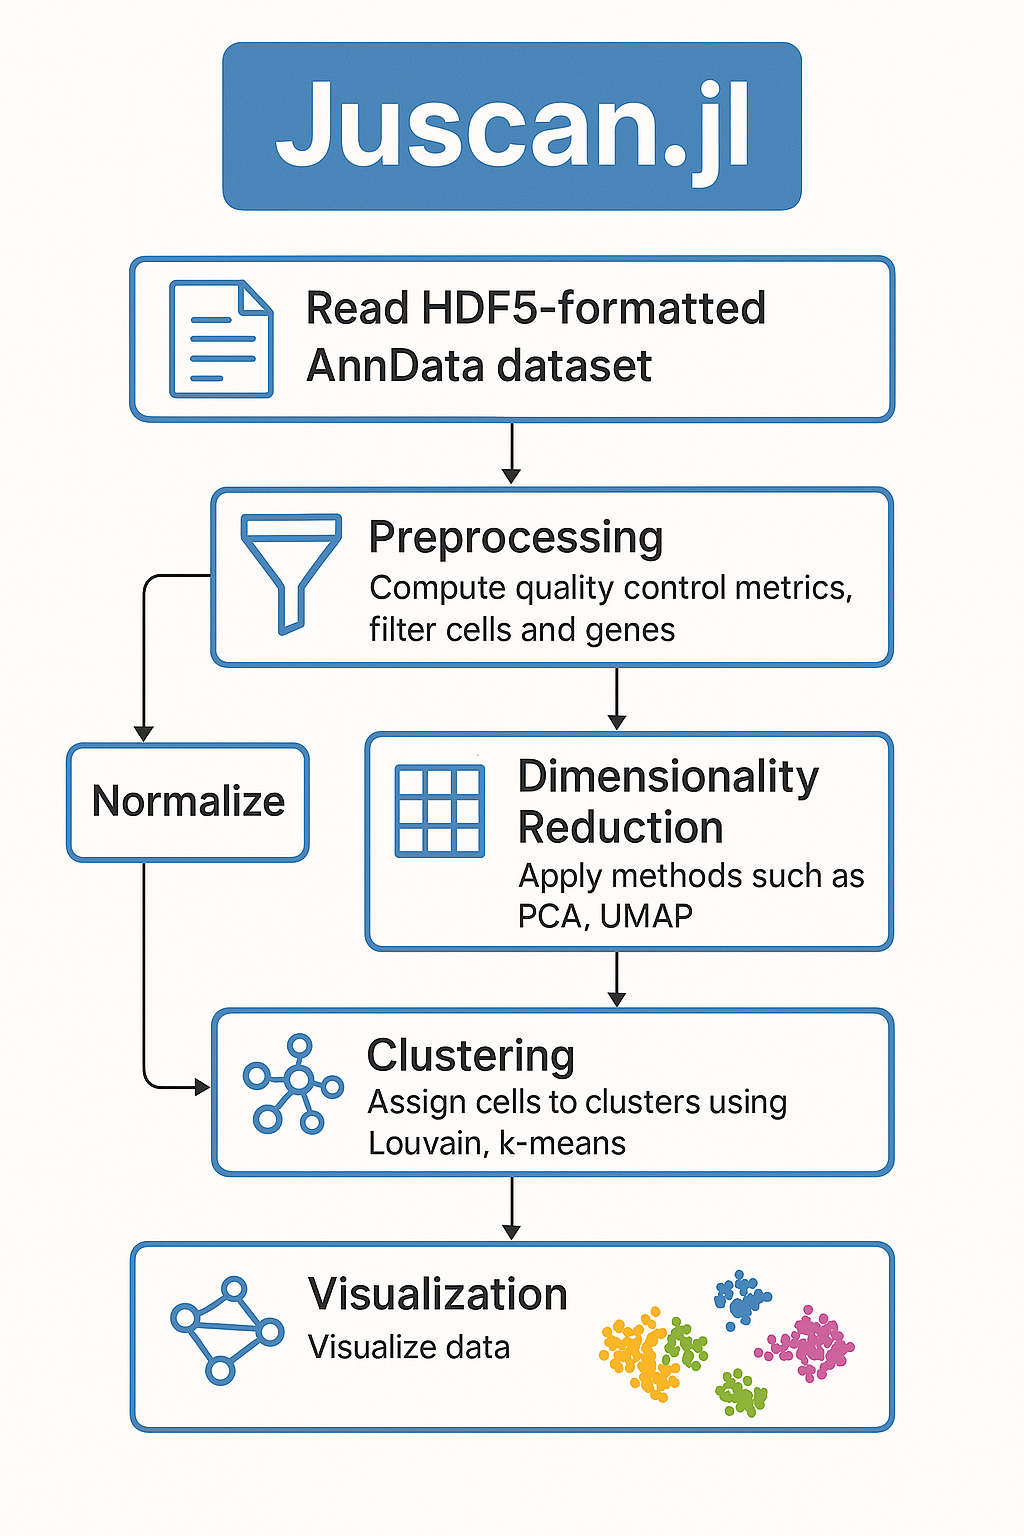
\includegraphics[width=0.4\textwidth]{img/flow_chart.png}
  \caption{Juscan.jl流程图}
  \label{img:flow}
\end{figure}

\subsection{系统模块划分}

如代码\ref{code:文件结构},此平台使用模块化的设计,将不同的功能划分到各自所属的模块中,以提高代码的整洁性、可维护性和扩展能力。

\begin{fancybox}{文件结构}
\addcontentsline{lot}{table}{代码~\thetcbcounter: 文件结构}
\begin{lstlisting}[numbers=none]
  Juscan.jl/
  ├── src/
  │   ├── preprocessing/
  │   │   ├── filter.jl                   # filter cells and genes
  │   │   ├── normalization.jl            # data normalization methods
  │   │   ├── pp.jl                       # preprocessing module
  │   │   ├── qc.jl                       # quality control methods
  │   │   └── utils.jl
  │   ├── tools/
  │   │   ├── cluster.jl                  # clustering methods
  │   │   ├── hvg.jl                      # highly variable genes
  │   │   ├── louvain.jl                  # louvain clustering
  │   │   ├── modularityClustering.jl     # modularity clustering
  │   │   ├── pca.jl                      # dimensionality reduction
  │   │   ├── snn.jl                      # SNN neighbour
  │   │   └── tl.jl                       # tools 
  │   ├── plots/
  │   │   ├── colors.jl
  │   │   ├── pl.jl
  │   │   └── plots.jl
  │   ├── Juscan.jl                       # Main module file
  │   ├── anndata.jl                      # anndata utilities
  │   └── utils.jl
  ├── docs/                               # documentation directory
  ├── test/                               # unit test directory
  ├── LICENSE
  ├── Project.toml                        # Julia project files
  └── README.md
\end{lstlisting}
\end{fancybox}

整体的Juscan.jl主要分为文档文件夹,单元测试文件夹,以及源代码文件夹。

源代码文件夹中Juscan.jl为整个项目的主模块,为项目导入需要的依赖库,加载子模块,以及对外暴露API接口。

导入的子模块包括preprocessing, tools, plots, 分别为单细胞的分析提供预处理,主要分析算法与可视化。

本项目由\href{https://github.com/scverse/Muon.jl}{Muon.jl}提供官方的AnnData数据结构, 代码\ref{code:Muon.AnnData}代表了Muon.anndata基本结构。

\section{数据结构}

\begin{fancybox}{Muon.AnnData}
\addcontentsline{lot}{table}{代码~\thetcbcounter: Muon.AnnData}
\begin{lstlisting}[language=julia]
mutable struct AnnData <: AbstractAnnData
  file::Union{HDF5.File, HDF5.Group, Nothing}

  X::Union{AbstractMatrix{<:Number}, Nothing}

  obs::DataFrame
  obs_names::Index{<:AbstractString}

  var::DataFrame
  var_names::Index{<:AbstractString}

  obsm::StrAlignedMapping{Tuple{1 => 1}, AnnData}
  obsp::StrAlignedMapping{Tuple{1 => 1, 2 => 1}, AnnData}

  varm::StrAlignedMapping{Tuple{1 => 2}, AnnData}
  varp::StrAlignedMapping{Tuple{1 => 2, 2 => 2}, AnnData}

  layers::AbstractAlignedMapping{Tuple{1 => 1, 2 => 2}, String}

  uns::Dict{<:AbstractString, <:Any}
end
\end{lstlisting}
\end{fancybox}

\begin{figure}[htbp]
  \centering
  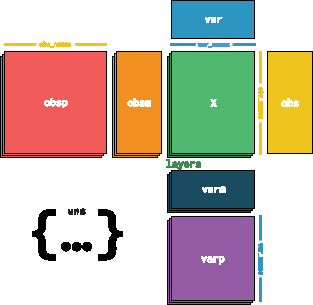
\includegraphics[width=0.5\textwidth]{img/anndata_schema.pdf}
  \caption{anndata数据结构示意图}
  \label{img:anndata}
\end{figure}


但是Muon.jl并没有提供足够多的处理anndata数据结构的方法行为,为了补充这方面的不足,本项目在\lstinline|src/anndata.jl|文件中进行了一些简单的扩充,包括子集化,插入观测与特征数据框,获取与设观测值的各个维度等方法。

\section{数据预处理模块}

\subsection{计算质量控制指标}

为了评估单细胞或多组学数据中的细胞与基因质量,我们实现了一个模块化的质量控制(quality control, QC)指标计算函数 \code{calculate_qc_metrics}。该函数支持从不同表达矩阵源(如主矩阵、原始计数矩阵 \code{adata.raw.X} 或指定的 \code{layer})提取表达数据,并分别计算细胞和基因层面的多种常用 QC 指标。

该函数的调用格式如下:

\begin{fancybox}{Muon.Pp.calculateQcMetrix}
\addcontentsline{lot}{table}{代码~\thetcbcounter: Muon.Pp.calculate\_qc\_metrix}
\begin{lstlisting}[language=julia]
calculate_qc_metrics(
  adata;
  expr_type="counts",
  var_type="genes",
  qc_vars=String[], 
  percent_top=[50, 100, 200, 500],
  layer=nothing,
  use_raw=false, 
  use_log1p=true,
  parallel=nothing
)::Tuple{DataFrame, DataFrame}
\end{lstlisting}
\end{fancybox}

在细胞维度上,函数会统计每个细胞中被检测到的特征数量、总表达量、log 转换后的表达水平、以及前若干高表达基因(如前 50、100、200 和 500 个)所占的表达比例。此外,用户可通过 \code{qc_vars} 参数指定一组具有特殊生物学意义的基因类别(如线粒体基因、核糖体基因等),函数将进一步评估这些类别基因在各细胞中的表达总量和比例。

在基因维度上,函数则计算每个基因在细胞群体中的检测频率、平均表达水平、零表达比例(dropout rate)以及总表达量等指标。这些指标可用于后续的基因过滤与特征选择。

函数 \code{calculate_qc_metrics} 返回两个 \code{DataFrame} 对象,分别包含细胞与基因层面的 QC 指标;而对应的 \code{calculate_qc_metrics!} 则为原地版本,直接将计算结果存储于 \code{adata.obs} 与 \code{adata.var} 字段中,便于与后续分析模块协同使用。

为支持灵活的数据接口设计,该模块还实现了表达矩阵的抽象选择函数 \code{_choose_mtx_rep},并对核心 QC 计算逻辑进行了进一步拆分,分别实现了用于细胞维度的 \code{describe_obs}/\code{describe_obs!} 和基因维度的 \code{describe_var}/\code{describe_var!}。其中,top-n 表达占比的计算由辅助函数 \code{top_segment_proportions} 实现。

该模块参考了 Scanpy 与 Seurat 的 QC 实践流程,并结合 Julia 类型系统设计了更高的通用性与可组合性,便于集成到多模态数据分析管线中。

\subsection{过滤}

在质量控制指标计算之后,我们进一步对数据进行细胞与基因的过滤,以剔除潜在的低质量条目,减少技术噪声对下游分析的干扰。本研究实现了一套通用的过滤函数,支持以总表达量、检测到的基因数(或细胞数)为阈值,灵活筛选细胞或基因,如代码\ref{code:Muon.Pp.filter}。

\begin{fancybox}{Muon.Pp.filter}
\addcontentsline{lot}{table}{代码~\thetcbcounter: Muon.Pp.filter}
\begin{lstlisting}[language=julia]
filter_cells!(
  data::Muon.AnnData;
  min_counts=nothing, min_genes=nothing,
  max_counts=nothing, max_genes=nothing
)::Nothing
filter_genes!(
  data::Muon.AnnData;
  min_counts=nothing, min_cells=nothing,
  max_counts=nothing, max_cells=nothing
)::Nothing
\end{lstlisting}
\end{fancybox}

细胞过滤函数 \code{filter_cells} 支持以下常用策略:

  \begin{itemize}
    \item 最小/最大总表达量(\code{min_counts}, \code{max_counts})
    \item 最小/最大检测基因数(\code{min_genes}, \code{max_genes})
    \item 可选择返回布尔向量(用于掩码子集)或过滤后的新对象(通过设置 \code{copy=true})
    \item 同时提供 \code{filter_cells!} 实现原地修改。
  \end{itemize}

类似地,基因过滤函数 \code{filter_genes} 支持以以下标准筛选:

  \begin{itemize}
    \item 被表达的细胞数量阈值(\code{min_cells}, \code{max_cells})
    \item 总表达量阈值(\code{min_counts}, \code{max_counts})
    \item 同样支持返回掩码或直接修改 \code{AnnData} 对象
  \end{itemize}

为确保操作语义明确,所有函数均要求每次仅传入一个过滤标准,以避免混淆。被筛选出的条目数量将在控制台输出日志,便于用户了解过滤效果。

该模块基于 Juscan.subset\_adata! 接口统一实现子集化操作,保证了代码的可维护性与高一致性,可无缝集成至数据预处理工作流中。

\subsection{归一化}


为消除不同细胞测序深度(即总 UMI 数)差异所带来的偏倚,我们实现了一个可扩展的总表达量归一化函数 \code{normalize_total},用于将每个细胞的表达矩阵缩放至统一的目标总量。该方法类似于 Scanpy 中的 \code{normalize_total} 或 Seurat 中的 \code{NormalizeData},但更具灵活性与模块化。

\begin{fancybox}{Muon.Pp.normalize}
\addcontentsline{lot}{table}{代码~\thetcbcounter: Muon.Pp.normalize}
\begin{lstlisting}
normalize_total(
    adata::AnnData;
    target_sum::Union{Real, Nothing}=nothing,
    exclude_highly_expressed::Bool=false,
    max_fraction::Float64=0.05,
    key_added::Union{String, Nothing}=nothing,
    layer::Union{String, Nothing}=nothing,
    layers::Union{String, Vector{String}, Nothing}=nothing,
    layer_norm::Union{String, Nothing}=nothing,
    copy::Bool=false
)::Union{AnnData, Dict{String, Any}}
normalize_total!(
    adata::AnnData;
    target_sum::Union{Real, Nothing}=nothing,
    exclude_highly_expressed::Bool=false,
    max_fraction::Float64=0.05,
    key_added::Union{String, Nothing}=nothing,
    layer::Union{String, Nothing}=nothing,
    layers::Union{String, Vector{String}, Nothing}=nothing
)::Nothing
\end{lstlisting}
\end{fancybox}

该函数通过计算每个细胞的总表达量(按行求和)作为归一化因子,并将表达矩阵按比例缩放,从而实现标准化。若未指定目标值(\code{target_sum}),则默认将每个细胞归一化至群体中位总表达量。此外,函数允许用户通过参数 \code{exclude_highly_expressed} 排除在某些细胞中高度表达的基因(如线粒体或核糖体基因),避免其对归一化因子的主导效应。

我们提供了两种版本的归一化函数:

    \code{normalize_total}:返回归一化后的新对象或结果字典;

    \code{normalize_total!}:原地(in-place)修改原始数据结构,节省内存。

这两个函数均支持对单个 \code{layer} 或多个 \code{layers} 进行归一化操作,并可通过参数 \code{layer_norm} 控制不同层归一化的参考因子。此外,归一化因子也可通过 \code{key_added} 参数保存至 \code{adata.obs} 中,用于后续批量分析或可视化。

值得注意的是,对于表达全为零的细胞,函数会发出警告提示。我们建议在归一化之前结合质量控制结果,先剔除此类无信息细胞。

\section{工具模块}

\subsection{高可变基因}

在单细胞 RNA 测序分析中,高变异基因(highly variable genes, HVGs)的识别对于后续的降维、聚类与轨迹推断等分析具有重要意义。为此,我们基于 Seurat v3 的策略,在 Julia 中实现了一套高变基因筛选模块 \code{highly_variable_genes},该方法兼容批次(batch-aware)处理,适用于多样本或多组学场景下的高变基因筛选。

该方法首先对每个批次独立计算每个基因的平均表达量与方差,并通过 LOESS 回归(局部加权多项式拟合)建模均值-方差关系,获得期望方差。随后,对原始方差进行校正,计算归一化后的方差作为变异性的衡量指标。对于跨多个批次的分析,方法进一步对各批次筛选结果进行合并,通过多批次中位排名的方式选出最终的一组 HVGs,保证其在多个批次中稳定地表现出高变异性。

我们实现了以下三类函数接口:

    % \code{highly_variable_genes}:返回 HVG 信息的 \code{DataFrame},不修改原始数据;
    % \code{highly_variable_genes!}:原地执行 HVG 计算,并将结果添加到 \code{adata.var};
    % \code{subset_to_hvg!}:在执行 HVG 筛选后,将数据集子集化,仅保留被识别为高变异的基因。
\begin{fancybox}{Muon.Tl.hvg}
\addcontentsline{lot}{table}{代码~\thetcbcounter: Muon.Tl.highly\_variable\_genes}
\begin{lstlisting}
subset_to_hvg!(adata::AnnData;
  layer::Union{String,Nothing} = nothing,
  n_top_genes::Int=2000,
  batch_key::Union{String,Nothing} = nothing,
  span::Float64=0.3,
  verbose::Bool=true
)
highly_variable_genes(adata::AnnData;
  layer::Union{String,Nothing} = nothing,
  n_top_genes::Int=2000,
  batch_key::Union{String,Nothing} = nothing,
  span::Float64=0.3
)
highly_variable_genes!(adata::AnnData;
  layer::Union{String,Nothing} = nothing,
  n_top_genes::Int=2000,
  batch_key::Union{String,Nothing} = nothing,
  span::Float64=0.3,
  replace_hvgs::Bool=true,
  verbose::Bool=false
)
\end{lstlisting}
\end{fancybox}

函数输出包括每个基因的均值、方差、归一化方差、在多个批次中的高变频次,以及最终的变异性排名。若数据中已有 HVG 注释,用户可选择是否替换(\code{replace_hvgs=true})。

\subsection{降维}

我们首先实现了 \code{log_transform!} 与 \code{logp1_transform!} 函数,用于对数据执行 $\log(x + \varepsilon)$ 或 $\log(1 + x)$ 变换,以增强表达量在低值区间的分布分辨能力。默认会将结果保存至新的数据层,便于复用与回溯。此外,函数 \code{standardize} 与 \code{prcomps} 封装了标准化与主成分提取过程,提供更底层的控制接口。

\subsubsection{(1)pca}

函数 \code{pca!} 实现了对 \code{AnnData} 对象中指定数据层的 PCA 计算,并将结果存储于 \code{adata.obsm["PCA"]} 中,供后续分析调用。该函数支持自动寻找合适的输入表达矩阵:若未提供目标数据层,则会依次查找是否存在经过对数转换的表达矩阵(\code{"log_transformed"})或归一化数据层(\code{"normalized"});若均不存在,则自动执行归一化与对数转换流程。

\begin{fancybox}{Muon.Tl.pca}
\addcontentsline{lot}{table}{代码~\thetcbcounter: Muon.Tl.pca}
\begin{lstlisting}
pca!(
  adata::Muon.AnnData;
  layer::String="log_transformed",
  n_pcs::Int=1000,
  verbose::Bool=true
)
\end{lstlisting}
\end{fancybox}

为确保主成分数量的合理性,函数会根据数据矩阵的维度自动调整主成分数量(\code{n_pcs}),避免维度溢出问题。计算过程采用稠密矩阵的奇异值分解(SVD)或稀疏矩阵的截断 SVD(TSVD),以兼容不同规模数据。

\subsubsection{(2)umap}

\begin{fancybox}{Muon.Tl.umap}
\addcontentsline{lot}{table}{代码~\thetcbcounter: Muon.Tl.umap}
\begin{lstlisting}
umap!(
  adata::Muon.AnnData;
  layer::String="log_transformed",
  use_pca_init::Bool=false,
  n_pcs::Int=100,
  verbose::Bool=true,
  kwargs...
)
\end{lstlisting}
\end{fancybox}

函数 \code{umap!} 用于计算数据的 UMAP 嵌入,并将结果包括嵌入坐标、最近邻索引、距离矩阵与模糊邻接图分别存入 \code{adata.obsm} 与 \code{adata.obsp} 中。该函数支持两种初始化方式:

\begin{itemize}
  \item 直接嵌入:使用指定数据层或自动生成的对数转换数据
  \item PCA 初始化:通过设置 \code{use_pca_init=true},先执行 PCA 作为初始嵌入向量
\end{itemize}

UMAP本身使用\code{UMAP.jl}实现,默认基于余弦距离构建邻接图,并可通过传入关键字参数(如 \code{n_neighbors}, \code{min_dist} 等)实现参数化控制。

\subsection{聚类}

聚类分析是单细胞数据中识别细胞亚群结构的关键步骤。此部分代码部分参考\code{ASCT.jl}的实现方法\upcite{Yang2023.12.27.573479}, 对\code{Muon:Ammdata}数据结构进行两类聚类方法:图结构驱动的模块度聚类(modularity clustering)与基于中心点的 KMedoids 聚类(近似 KMeans),构成了双路径的细胞聚类框架。为了便于用户在不同分析阶段调用聚类方法,我们提供了统一接口 clustering!,支持多种参数配置与算法选择。

\begin{fancybox}{Muon.Tl.Clustering}
\addcontentsline{lot}{table}{代码~\thetcbcounter: Juscan.Tl.Clustering}
  \begin{lstlisting}
function clustering!(
  data::Muon.AnnData;
  method::AbstractString="mc",
  reduction::Union{AbstractString, Symbol}=:auto,
  use_pca::Union{AbstractString, Integer}="pca_cut",
  # n_pcs::Union{Integer, AbstractString}=5,
  tree_K::Integer=20,
  resolution::Union{Symbol, Real, AbstractRange}=:auto,
  cluster_K::Union{Nothing, Integer}=nothing,
  cluster_K_max::Union{Nothing, Integer}=30,
  dist::AbstractString="Euclidean",
  network::AbstractString="SNN",
  random_starts_number::Integer=10,
  iter_number::Integer=10,
  prune::AbstractFloat=1 / 15,
  seed::Integer=-1,
)
  \end{lstlisting}
\end{fancybox}

对\code{AnnData}对象执行聚类分析,结果会自动保存在\code{adata.obs}中。该函数根据参数\code{method}选择不同的聚类策略。

\textbf{a.~基于模块度的图聚类(modularity clustering)}

该方法通过构建细胞的共享最近邻图(Shared Nearest Neighbor, SNN),并以最大化模块度(modularity)为目标,对细胞图进行社团划分。方法流程如下:

\begin{enumerate}
  \item 图构建:在降维空间(如 PCA)中,使用 KD 树加速寻找每个细胞的 $K$ 个近邻,构建 KNN 或 SNN 图。SNN 图定义如下:

\begin{equation}
  \text{SNN}_{ij} = |\mathcal{N}_i \cap \mathcal{N}_j| / K
\end{equation}

其中 $\mathcal{N}_i$ 表示细胞 $i$ 的邻居集合。

\item 图稀疏化与剪枝:通过阈值参数 $\alpha \in (0, 1]$ 对图进行稀疏化,仅保留重叠度高的邻接关系,以提高模块度检测的稳定性。

\item 模块度优化聚类:通过 Louvain 或 Leiden 等算法,在图中最大化以下模块度函数:

\begin{equation}
Q = \frac{1}{2m} \sum_{i,j} \left( A_{ij} - \gamma \frac{k_i k_j}{2m} \right) \delta(c_i, c_j)
\end{equation}

其中 $A_{ij}$ 为图邻接矩阵,$k_i$ 为节点度,$\gamma$ 为分辨率参数,$\delta$ 为 Kronecker delta。我们支持不同的 $\gamma$ 参数进行多分辨率扫描,自动推荐最优分辨率。

\end{enumerate}

\textbf{b.~基于KMedoids的中心点聚类(k-medoids clustering)}

KMedoids 聚类是一种鲁棒于异常值的变体,相较于 KMeans 选择“簇中心”,KMedoids 选择实际数据点作为中心。我们实现如下自动聚类过程:

\begin{enumerate}
  \item 距离计算:用户可选择多种距离度量,如欧氏距离、余弦距离、相关距离等,在降维空间中计算细胞间距离矩阵。

  \item 自动选择簇数 $K$:

  \begin{itemize}
    \item 计算多个 $K$ 值下的聚类结果(并行加速);
    \item 对每个聚类结果,计算 silhouette 系数 $\bar{s}$ 与标准差;
    \item 同时评估总成本的肘部法则(elbow method);
    \item 综合两个指标,自动选择最优 $K$ 值:
  \end{itemize}

\end{enumerate}

\begin{equation}
K^* = \arg\max_K \left( \text{silhouette score} - \text{total cost deviation} \right)
\end{equation}

\section{可视化模块}

单细胞组学分析常涉及高维数据的降维、聚类和分类结果,为了更好地呈现这些复杂结构,我们在 \code{Juscan.Plots} 中实现了一套基于 \code{CairoMakie} 的绘图模块,涵盖多种用于探索性分析与结果展示的图形函数。该模块强调高可配置性、视觉一致性与图像质量,便于科研报告与论文作图。

\subsection{调色机制与主题色板}

我们设计了一套模块化的调色系统,通过 \code{get_palette} 和 \code{get_continuous_colormap} 接口,提供一系列离散与连续的调色方案,支持自动扩展与下采样。其中,离散色板如 \code{"friendly"}、\code{"apple"}、\code{"rainbow"} 等适用于类别标签着色,而连续色带则集成自 \code{ColorSchemes.jl},可用于表达量、主成分值等数值信息的可视化。所有色板均通过自定义函数实现扩展与裁剪策略,确保图形风格在多图展示中保持一致。

\subsection{可视化函数接口}

模块当前提供以下核心函数:

\begin{itemize} \item \code{violin}:绘制提琴图,展示多个观测变量(如基因表达、细胞指标)的分布,支持点抖动(jitter)与多子图并排布局。 \item \code{scatter}:绘制二维散点图,支持根据第三变量进行着色(如根据表达量、UMAP/PCA位置等变量上色)。 \item \code{hvg_scatter}:用于展示高变异基因的筛选结果,通过平均表达与变异度关系图突出高变基因在全体中的位置。 \item \code{plot_variance_ratio}:绘制 PCA 主成分的方差解释比例图,支持对前若干主成分进行可视化,并自动标注前 5 个 PC。 \item \code{plot_umap}:绘制 UMAP 降维嵌入图,支持按照类别标签上色,自动生成图例并匹配色板风格。 \end{itemize}

\subsubsection{(1) violin:分布可视化}

该函数支持绘制多个变量在样本中的表达分布,可用于细胞质控指标(如总 UMI 数、线粒体比例)的展示。用户可指定色板名与透明度参数,自动匹配子图数量与调色方案。此外还可设置点抖动强度与保存图像路径:

\begin{fancybox}{Juscan.Plots.violin} 
  \addcontentsline{lot}{table}{代码~\thetcbcounter: Muon.Pl.violin}
  \begin{lstlisting} 
violin(
  adata::AnnData,
  keys::Union{String, Vector{String}};
  width::Real=600,
  height::Real=400,
  jitter::Union{Bool, Real}=0.5, dot_size::Real=2,
  title::String="violin plot",
  palette_name::String="friendly",
  fill_alpha::Real=1.0, 
  savefig::Union{Bool, String}=false
) 
  \end{lstlisting} 
\end{fancybox}

\subsubsection{(2) hvg\_scatter:高变基因展示}

为辅助用户评估 HVG 的筛选结果,我们实现了 \code{hvg_scatter} 函数,绘制均值-方差与归一化方差的二维图。灰色表示非 HVG 基因,黑色点表示已筛选出的 HVGs,有助于观察其在全体中的分布位置。

\subsubsection{(3) plot\_umap:嵌入可视化}

该函数根据 \code{adata.obsm} 中的 UMAP 坐标绘图,并根据 \code{adata.obs} 中的分类变量进行着色。支持自定义调色板、图形尺寸与图像保存路径:

\begin{fancybox}{Juscan.Plots.plot umap}
  \addcontentsline{lot}{table}{代码~\thetcbcounter: Muon.Pl.plot\_umap}
  \begin{lstlisting} 
plot_umap(
  adata;
  color_by::String="clusters_latest",
  key="umap",
  palette_name::String="rainbow",
  savefig::Union{Bool, String}=false
) 
  \end{lstlisting} 
\end{fancybox}

\subsubsection{(4) scatter 与 plot\_variance\_ratio}

除标准二维散点图外,我们也实现了用于主成分方差比分析的函数 \code{plot_variance_ratio}。其通过绘制 log 方差比图,帮助用户直观判断 PCA 的有效维度。


\chapter{实验与评估}
\section{实验流程}

\begin{figure}[H]
  \centering
  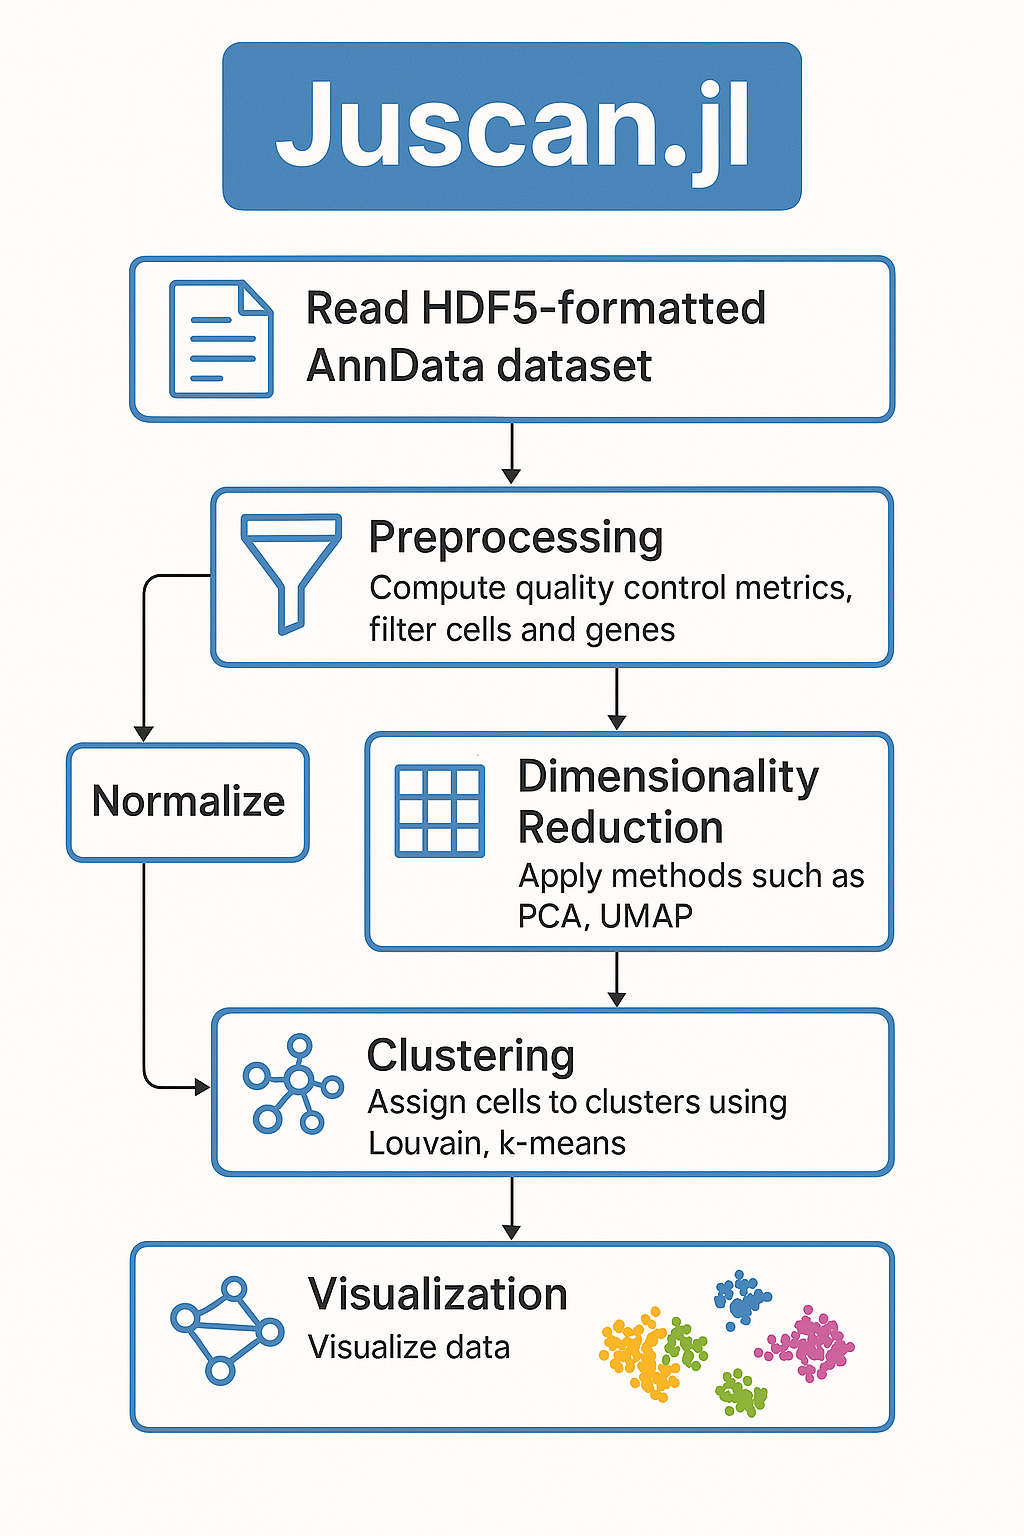
\includegraphics[width=0.57\textwidth]{img/flow_chart.png}
  \caption{实验流程}
  \label{fig:flow_chart}
\end{figure}

\section{实验方法}

\subsection{扩增插入基因}

\textbf{一、引物设计}

\begin{enumerate}[itemsep=0.1em]
\item 使用高质量的模板。
\item 勿使用dUTP和带有尿嘧啶的引物和模板。
\item 如实验需要,可适当提高Phanta酶的使用量,但50ul体系内酶量建议不要超过2ul。
\item Phanta酶具有较强的校对活性。因此,如扩增产物需要进行TA克隆,加之前必须进行DNA纯化。
\item 为了防止Phanta酶的校对活性降解引物,在配制反应体系时请最后加入聚合酶。
\item 引物设计
\begin{enumerate}[label={(\arabic*)}, itemsep=0.1em]
  \item 引物3端最后一个碱基最好为G或者C;
  \item 引物3端最后8个碱基应避免出现连续错配;
  \item 引物3端应避免出现发夹结构;
  \item 正向引物和反向引物的Tm值相差不超过1℃为佳,Tm值调整至55~65℃为佳;
  \item 引物额外附加序列,即与模板非配对序列,不应参与引物Tm值计算
  \item 引物的GC含量控制在40\%-60\%之间;
  \item 引物A、G、C、T整体分布要尽量均匀,避免使用GC或者AT含量高的区域;
  \item 引物内部或者两条引物之间避免有5个碱基以上的互补序列,两条引物的3端避免有3个碱基以上的互补序列;
  \item 引物设计完毕请使用NCBI BLAST功能检索引物特异性,以避免非特异性扩增产生。
\end{enumerate}
\end{enumerate}

\textbf{二、PCR}(Panta酶反应体系,从全基因组中PCR结束之后需要做一步消化。要注意全程在冰上操作,加的体积从大到小)

\begin{longtable}{cc}
  \caption{PCR 反应体系} \\
  \toprule
  \textbf{组分} & \textbf{体积} \\
  \midrule

  ddH$_2$O & 17~$\mu$l(加到 50~$\mu$l) \\
  2$\times$Buffer & 25~$\mu$l \\
  dNTP & 1~$\mu$l \\
  上、下游引物(分开加) & 2~$\mu$l \\
  酶 & 1~$\mu$l \\
  模板 DNA & 2~$\mu$l \\

  \bottomrule
\end{longtable}


\begin{longtable}{ccc}
  \caption{PCR 反应条件} \\
  \toprule
  \textbf{步骤} & \textbf{时间} & \textbf{温度} \\
  \midrule
  \endfirsthead

  \multicolumn{3}{l}{\textit{续表:PCR 反应条件}} \\
  \toprule
  \textbf{步骤} & \textbf{时间} & \textbf{温度} \\
  \midrule
  \endhead

  \bottomrule
  \multicolumn{3}{r}{\textit{表格接下页}} \\
  \endfoot

  \bottomrule
  \endlastfoot

  预变性 & 3 min & 95$^\circ$C \\
  变性   & 15 sec & 95$^\circ$C \\
  退火   & 15 sec & 60$^\circ$C(根据引物 Tm 值调整) \\
  延伸   & 150 sec(根据 bp 长度调整) & 72$^\circ$C \\
  彻底延伸 & 5 min & 72$^\circ$C \\

\end{longtable}

\textbf{三.跑胶}

\begin{enumerate}[itemsep=0.1em]
  \item 安仪器,根据要跑胶的基因数目的具体情况计算要用到的梳子种类和皿的种类。
  \item 加溶剂,两次煮沸,在侧面冷水下冲洗到$50^\circ\text{C}$。
  \item 加核酸染料。
  \item 倒胶。
  \item 晾干30min,待胶条凝固冷却成型。
  \item 取梳子。
  \item 转胶条。
  \item 加基因和marker。
  \item 电压150V,电流400A,跑胶。
\end{enumerate}

\textbf{四.胶回收}

\begin{enumerate}[itemsep=0.1em]
  \item 切胶,置于2.0ml EP管中。切胶要放切胶板,切完的胶扔到红色垃圾袋,管中的胶放在相应的引物旁边,作好引物名称标记。
  \item 加3倍凝胶体积的Buffer MB,$55^\circ\text{C}$水浴加热,直至凝胶全部融化。
  \item 在等待胶溶期间,向离心吸附柱中加入500$\mu$l Buffer BL,静止1min,室温下12,000rpm离心1min,弃收集管中的废液,将离心吸附柱重新放回收集管中。
  \item 待凝胶溶液冷却至室温后,转移到离心吸附柱内,静置1min,室温下12,000rpm离心1min。
  \item 弃除收集管中的废液,将离心吸附柱重新插回收集管中。
  \item 加入600$\mu$l Buffer MW于离心吸附柱中,室温下12,000rpm离心30s,弃除收集管中的废液,将离心吸附柱重新插回收集管中。
  \item 重复操作步骤6。
  \item 室温下12,000rpm空离2min,弃除收集管。
  \item 将吸附柱置于1.5ml离心管中,加入50$\mu$l\~100$\mu$l至吸附柱中央,室温静置1min,12,000rpm离心1min。
  \item 弃去吸附柱,获得的DNA片段可直接用于后续反应或于$-20^\circ\text{C}$长期保存。
\end{enumerate}

\subsection{扩增质粒}

\textbf{一.摇菌(扩增质粒数量)}

\textbf{二.提质粒}

\begin{enumerate}[itemsep=0.3em]
  \item 取摇菌管,4000rpm离心3min。弃去培养基,将摇菌管倒扣于吸水纸上吸尽残液。
  \item 向留有菌体沉淀的摇菌管中加入250$\mu$l Buffer P1,用移液器或涡旋振荡混匀后将其转入1.5ml离心管中。
  \item 向步骤2中加入250$\mu$l Buffer P2,温和地上下颠倒混匀8–10次,使菌体充分裂解。
  \item 向步骤3中加入350$\mu$l Buffer P3,立即温和地上下颠倒8–10次使溶液彻底中和。将混合液加入吸附柱中,12,000rpm离心30–60s,弃废液并将吸附柱重新放回收集管中。
  \item 重复步骤4。
  \item 将吸附柱放入新的1.5ml离心管中,12,000rpm离心2min,以干燥吸附柱,彻底去除残留漂洗液。
  \item 将吸附柱再次置于新的灭菌1.5ml离心管中,加入30$\mu$l无菌水至吸附柱膜中央,室温静置2min,12,000rpm离心1min以洗脱DNA。
  \item 测定质粒DNA浓度,并在离心管上做好标记。
\end{enumerate}

\subsection{构建新的质粒}

\textbf{一、酶切}

\begin{longtable}{cc}
  \caption{酶切体系} \\
  \toprule
  \textbf{组分} & \textbf{用量} \\
  \midrule
  \endfirsthead

  \multicolumn{2}{l}{\textit{续表:酶切体系}} \\
  \toprule
  \textbf{组分} & \textbf{用量} \\
  \midrule
  \endhead

  \bottomrule
  \endfoot

  \bottomrule
  \endlastfoot

  Plasmid & 2~$\mu$g \\
  Enzyme 1 & 1~$\mu$l \\
  Enzyme 2 & 1~$\mu$l \\
  10$\times$酶切 Buffer & 3~$\mu$l \\
  ddH$_2$O & up to 30~$\mu$l \\
  
\end{longtable}

震荡混匀,37$^\circ\text{C}$酶切30min(3000bp酶切30min)

\textbf{二、纯化}(与胶回收的原理和步骤类似)

\textbf{三、连接}

弹管混匀后冰浴30min

\begin{longtable}{cc}
  \caption{连接体系} \\
  \toprule
  \textbf{组分} & \textbf{用量} \\
  \midrule
  \endfirsthead

  \multicolumn{2}{l}{\textit{续表:连接体系}} \\
  \toprule
  \textbf{组分} & \textbf{用量} \\
  \midrule
  \endhead

  \bottomrule
  \endfoot

  \bottomrule
  \endlastfoot

  载体 & 30~ng(3~$\mu$l / 2~$\mu$l) \\
  插入序列 & 50~ng(5~$\mu$l / 6~$\mu$l) \\
  10$\times$酶切 Buffer & 1~$\mu$l \\
  Exo3 & 1~$\mu$l(取 1~$\mu$l 加到 9~$\mu$l 水中,稀释 10 倍后取 1~$\mu$l) \\
\end{longtable}

\textbf{四.转化}

\begin{enumerate}[itemsep=0.1em]
  \item 取感受态细胞放冰上解冻。
  \item 向感受态细胞中加入10$\mu$l连接产物,弹管混匀。
  \item 冰浴10min。
  \item 42$^\circ$\text{C}热激90s。
  \item 冰浴3\~5min。
  \item 在超净台中加入1ml不含抗生素的LB培养基,混匀后于37$^\circ$\text{C}孵育1h。
  \item 5,000rpm离心4min,吸走上清,只留100$\mu$l,吹打重悬后涂布于抗性平板上。
  \item 置于37$^\circ$\text{C}培养10–16h。
  \item 挑取单克隆接种至含抗生素的LA液体培养基中,小摇培养约3h。
\end{enumerate}

\textbf{注意:}需要设置一个阴性对照——酶切后的载体(3$\mu$l,无需添加连接酶),用于判断载体是否被完全切开或发生自我连接。

\subsection{PCR 验证和测序}

\textbf{一、菌液PCR}

\textbf{二、跑胶验证}

\subsection{RNAi 实验}

\begin{enumerate}[itemsep=0.3em]

  \item 第0天:在含抗生素的LB液体培养基中接种含有RNAi质粒的HT115大肠杆菌,于37$^\circ$\text{C}震荡培养12–16小时,以获取最多的活菌。
  
  \item 第一天:
  \begin{enumerate}[label*={(\alph*)}, itemsep=0.3em]
    \item 将菌液1:100稀释至2$\times YT ^+$ 抗生素中,培养至OD$_{595}$ = 0.4;
    \item 加入无菌 IPTG 使终浓度达到0.4mM,在37$^\circ$\text{C}摇床诱导4小时;
    \item 在含抗生素和IPTG的培养条件下继续培养。可直接使用培养液,也可将菌液以2000rpm离心、吸走上清后重悬浓缩细胞,然后播种至RNAi平板上。
  \end{enumerate}
  
  \item 挑选线虫至RNAi平板上,开始RNAi实验。
  
\end{enumerate}

\subsection{Smurf Assy 实验}

\begin{enumerate}[itemsep=0.1em]
  \item 提前一天使用LB培养基摇菌OP50(线虫的食物),于37$^\circ$\text{C}培养12–16小时。使用前将菌液浓缩10倍。
  \item 配制5\% Smurf染液:在浓缩后的菌液中加入0.25g Smurf染料粉末,加入5ml浓缩菌液,涡旋混匀备用。
  \item 用2ml离心管,加入200$\mu$l M9缓冲液,将待处理线虫挑入管中。再加入400$\mu$l步骤2中配制的5\% Smurf染液。
  \item 将混合液放置在20$^\circ$\text{C}水平摇床上,缓慢摇晃3小时。
  \item 使用台式小型离心机离心10s,使线虫沉降至管底。吸去上清,保留约300$\mu$l液体,补加1ml M9,轻轻重悬清洗。重复洗涤多次,直到线虫体表的蓝色染料明显变淡,能透过离心管看到手指为止。最后保留约300$\mu$l液体。
  \item 将洗后的线虫液体,用低吸附枪头滴加在已吹干的NGM平板上,轻轻摇晃,使液体尽可能摊平于平板表面。从该平板中挑取线虫转移到无菌NGM平板(用于拍照)。
  \item 在无菌NGM平板上加入叠氮化钠杀死线虫,排列整齐后进行拍照观察。根据Smurf染料在虫体内的渗透程度,判断线虫肠道屏障的完整性。
\end{enumerate}

\subsection{荧光共聚焦实验}


\begin{enumerate}[itemsep=0.1em]
\item 使用左旋咪唑麻醉线虫,将线虫进行排列(每个RNAi组拍摄大约30条虫子)。
\item 使用488nm波长的荧光通道,拍摄线虫表皮细胞间HMR-1-GFP的点状荧光信号。
\end{enumerate}

\section{小结}

本章节详细描述了从基因扩增到荧光共聚焦实验的完整实验步骤,涵盖了DNA操作,RNAi实验以及线虫屏障相关实验多个环节。整个实验流程设计严谨,步骤清晰,我们的实验确保了每一步操作的准确性和可重复性,为研究基因功能和线虫生物学特性提供了可靠的实验方法。

我们的实验首先从引物设计开始,整个引物设计规则严谨,为了确保后续的一系列实验按部就班开展。在扩增插入基因时,我们使用Phanta酶进行PCR反应, PCR产物会通过跑胶和胶回收进行纯化。接下来是质粒的扩增和提取。我们通过摇菌培养细菌以扩增质粒数量,然后进行质粒提取,最终获得高纯度质粒DNA。在构建新的质粒时,我们首先对质粒进行酶切,酶切后的载体通过纯化去除杂质,然后与插入目的片段进行连接,连接产物又通过转化进入感受态细胞,经过培养后在氨苄板上筛选阳性克隆。为了验证阳性克隆,本实验采用菌液PCR和跑胶验证,以确保插入序列的正确性。

随后我们进行RNAi实验。首先我们在LB培养基中培养HT115菌株,加入IPTG诱导dsRNA表达涂板。然后我们将线虫转移到RNAi平板上进行喂养。Smurf Assay实验用于评估线虫肠道屏障功能,利用浓缩菌液配制5\%的 Smurf染料,对线虫进行染色后通过离心、洗涤和显微镜观察得出线虫肠道屏障损伤程度结果。最后,荧光共聚焦拍摄和判断线虫表皮屏障的受损情况。最后两种判断线虫屏障受损与否的实验结果我们都将用定量软件进行分析,以确保最终的实验结论严谨可靠。


\chapter{讨论}
%%% 讨论

\section{研究成果总结}

本研究基于 Julia 编程语言成功设计并实现了一个高性能的单细胞数据分析平台 —— Juscan.jl。该平台以 Muon.jl 所提供的 AnnData 数据结构为核心,复刻并优化了 Scanpy 在 Python 生态中的分析流程,完成了从数据质量控制、标准化、高变基因筛选、降维、聚类到可视化的完整管线,构建出一个功能完备、接口友好、计算高效的分析框架。

更重要的是,Juscan.jl 采用模块化设计,具有良好的可扩展性和可维护性,为后续的算法开发和功能拓展提供了坚实的基础。

\section{未来工作展望}


尽管 Juscan.jl 已实现了基础的单细胞分析功能,但作为一个初步探索性的项目,仍存在许多可提升的方向,具体包括以下几个方面:

\begin{enumerate}
\item 多模态数据支持与整合: 当前版本主要面向 scRNA-seq 数据,未来可进一步支持 ATAC-seq、CITE-seq 以及空间转录组等多组学数据,并结合 Canonical Correlation Analysis、WNN等多模态聚类方法,实现更全面的细胞表征。
\item 更多聚类与轨迹推断算法的集成: 目前聚类模块仅支持 Louvain 与 k-medoids,后续可引入 Leiden 算法、基于高斯混合模型(GMM)的聚类方法,甚至构建基于图卷积神经网络(GCN)的聚类与分类器。同时,可引入 pseudotime 轨迹推断模块,满足发育过程建模的需求。
\item 计算性能的进一步优化: 尽管 Julia 语言本身具备极高的运行性能,但本项目中的部分性能瓶颈主要源于代码层面的实现尚不够成熟。例如,部分函数存在数据复制冗余、内存访问不充分优化、缺乏懒计算等问题,影响了整体的执行效率与稳定性。未来可以通过进一步剖析关键函数的瓶颈(如使用 @profile、@btime 等工具)、重构核心逻辑、合理安排内存布局、并结合并行/多线程机制等方式,显著提升 Juscan.jl 的运行效率与工程质量。同时,也可结合 PackageCompiler.jl 生成系统映像,以减少启动与冷启动时的性能损耗,从而带来更流畅的用户体验。
\item 用户交互体验与可视化增强: 当前可视化模块虽已支持 UMAP、提琴图等常规图形,但仍缺乏交互式浏览器支持。可借助 Makie.jl + Genie.jl 或 Pluto.jl 构建 Web 可视化平台,让用户通过图形界面进行数据探索。
\end{enumerate}


%=================================================================
%论文后部
\backmatter


%=======%
%引入参考文献文件
%=======%
\bibdatabase{bib/database}%bib文件名称 仅修改bib/ 后部分
\printbib
\nocite{*} %显示数据库中有的,但是正文没有引用的文献

\Appendix

\section{Juscan.jl源代码与文档}

源码见Github仓库: \href{https://github.com/zehua0417/Juscan.jl.git}{https://github.com/zehua0417/Juscan.jl.git}

其他更多使用细节见文档:\href{https://zehua0417.github.io/Juscan.jl/}{https://zehua0417.github.io/Juscan.jl/}

\section{性能检测}

\showcode{julia}{Juscan.jl速度检测}{../vs/src/sc.jl}
\showcode{R}{Seurat速度检测}{../vs/src/sc.R}
\showcode{python}{scanpy速度检测}{../vs/src/sc.py}

\Thanks

本论文的完成离不开多方的关心与支持,在此谨致以诚挚的感谢。

首先,衷心感谢我的导师赵伟老师在课题选题、研究设计与论文撰写过程中给予的悉心指导与宝贵建议。赵老师严谨治学的态度、敏锐的问题意识以及持续探索的精神,为本研究的顺利推进提供了重要保障。

感谢生命科学学院为我提供了良好的学习与科研环境,系统的课程设置与丰富的学术资源,为我的专业成长和科研训练打下了坚实基础。感谢各位授课教师在本科阶段的辛勤教学和耐心指导,使我得以不断夯实专业知识,拓展学术视野。

感谢我的家人长期以来给予的理解与支持,是他们无声的鼓励与陪伴,使我能够专注于学业,克服困难,坚定前行。

同时,感谢开源社区与相关软件项目开发者的无私贡献,特别是Muon.jl、Scanpy等项目,为本研究提供了重要的参考与技术支持。

最后,感谢在项目开发、测试与讨论过程中给予我帮助与建议的同学与朋友们。你们的支持使本项目不断完善,持续前进。

\Grade

\end{document}
